\documentclass{standalone} % DO NOT CHANGE THIS
\usepackage{tikz}
\usepackage[utf8]{inputenc}
\usepackage{graphicx}
\usepackage{times}
\usepackage{amssymb}
\usetikzlibrary[arrows.meta, positioning,math, calc, shapes.geometric,intersections, fit, backgrounds, decorations.pathmorphing]

\begin{document}

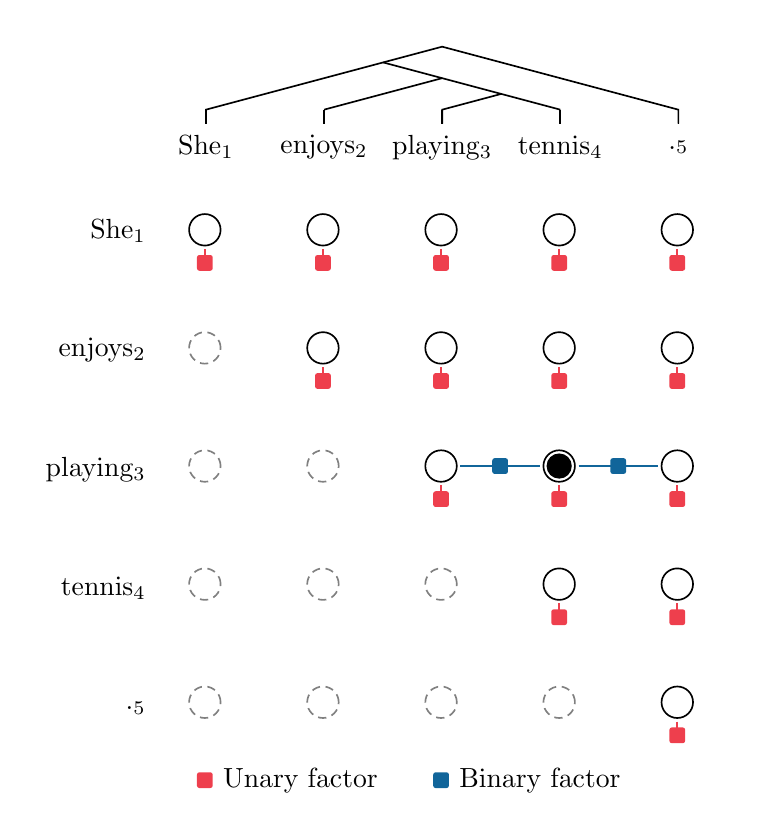
\begin{tikzpicture}[
        word/.style={
                minimum width=1.5cm,
                minimum height=1.5cm,
                inner sep=0pt,
                text width=1.5cm,
                % draw=black
            },
        red filled/.style={
                fill={rgb,255:red,238; green,63; blue,77},
            },
        blue filled/.style={
                fill={rgb,255:red,17; green,101; blue,154},,
            },
        red connect/.style={
                draw={rgb,255:red,238; green,63; blue,77},
                shorten >= 1pt,
                shorten <= 1pt,
                semithick
            },
        blue connect/.style={
                draw={rgb,255:red,17; green,101; blue,154},
                shorten >= 1pt,
                shorten <= 1pt,
                semithick
            },
        connect/.style={
                shorten >= -0.5pt,
                shorten <= 1pt,
            },
    ]
    \centering

    \node [word] [anchor=south west] (w00) {};
    \node [word] [anchor=north, align=right] (w01) at (w00.south) {She$_1$};
    \node [word] [anchor=north, align=right] (w02) at (w01.south) {enjoys$_2$};
    \node [word] [anchor=north, align=right] (w03) at (w02.south) {playing$_3$};
    \node [word] [anchor=north, align=right] (w04) at (w03.south) {tennis$_4$};
    \node [word] [anchor=north, align=right] (w05) at (w04.south) {.$_5$};
    \node [word] [anchor=south west, text centered, minimum height=0.6cm] (w10) at ($(w00.south east) + (1.5cm*0, 0)$) {She$_1$};
    \node [word] [anchor=south west, text centered, minimum height=0.6cm] (w20) at ($(w00.south east) + (1.5cm*1, 0)$) {enjoys$_2$};
    \node [word] [anchor=south west, text centered, minimum height=0.6cm] (w30) at ($(w00.south east) + (1.5cm*2, 0)$) {playing$_3$};
    \node [word] [anchor=south west, text centered, minimum height=0.6cm] (w40) at ($(w00.south east) + (1.5cm*3, 0)$) {tennis$_4$};
    \node [word] [anchor=south west, text centered, minimum height=0.6cm] (w50) at ($(w00.south east) + (1.5cm*4, 0)$) {.$_5$};


    \foreach \y in {1,...,5}
    \foreach \x in {\y,...,5} {
            \pgfmathtruncatemacro{\label}{\x*10 + \y}
            \node [circle,draw=black,semithick,inner sep=0pt,minimum size=0.4cm]  (w\x\y) at ($(w00.base) + (1.5cm*\x,-1.5cm*\y)$) {};
            \node [red filled,inner sep=0pt,minimum size=0.2cm,rounded corners=0.3mm]  (f\x\y) at ($(w\x\y) - (0, 0.42cm)$) {};
            \draw[red connect,thick,connect] (w\x\y.south) -- (f\x\y.north);
        }
    \foreach \x in {1,...,4}{
            \pgfmathtruncatemacro{\n}{\x + 1}
            \foreach \y in {\n,...,5}
                {\pgfmathtruncatemacro{\label}{\x*10 + \y}
                    \node [circle,draw=gray, densely dashed ,semithick,minimum size=0.4cm]  (w\x\y) at ($(w00.base) + (1.5cm*\x,-1.5cm*\y)$) {};}
        }
    \node [circle,draw=none,fill=black, inner sep=0pt, minimum height=0.32cm] at (w43) {};
    % \node [circle,draw=black,fill=black] at (w42) {};
    \draw[blue connect] (w33) -- (w43) node[midway,blue filled,inner sep=0pt,minimum size=0.2cm,rounded corners=0.3mm] {};
    \draw[blue connect] (w43) -- (w53) node[midway,blue filled,inner sep=0pt,minimum size=0.2cm,rounded corners=0.3mm] {};
    % \draw[blue connect] (w33) to [out=30, in=150] node[midway,blue filled,inner sep=0pt,minimum size=0.2cm,rounded corners=0.3mm] {} (w53) ;


    \node [] (c11) at ($(w10.center)+(0,0.6cm)$) {};
    \node [] (c22) at ($(w20.center)+(0,0.6cm)$) {};
    \node [] (c33) at ($(w30.center)+(0,0.6cm)$) {};
    \node [] (c44) at ($(w40.center)+(0,0.6cm)$) {};
    \node [] (c55) at ($(w50.center)+(0,0.6cm)$) {};
    \node [] (c34) at ($(w30.center)!0.5!(w40.center)+(0,0.8cm)$) {};
    \node [] (c24) at ($(w20.center)!0.5!(w40.center)+(0,1.0cm)$) {};
    \node [] (c14) at ($(w10.center)!0.5!(w40.center)+(0,1.2cm)$) {};
    \node [] (c15) at ($(w10.center)!0.5!(w50.center)+(0,1.4cm)$) {};
    \draw[semithick] ($(w10.center)+(0,0.3cm)$) -- (c11.south) -- (c14.south) -- (c15.south) -- (c55.south) -- ($(w50.center)+(0,0.3cm)$);
    \draw[semithick] ($(w30.center)+(0,0.3cm)$) -- (c33.south) -- (c34.south) -- (c44.south);
    \draw[semithick] (c14.south) -- (c24.south);
    \draw[semithick] (c22.south) -- (c24.south) -- (c34.south);
    \draw[semithick] (c11.south) -- ($(w10.center)+(0,0.3cm)$);
    \draw[semithick] (c22.south) -- ($(w20.center)+(0,0.3cm)$);
    \draw[semithick] (c33.south) -- ($(w30.center)+(0,0.3cm)$);
    \draw[semithick] (c44.south) -- ($(w40.center)+(0,0.3cm)$);
    \draw[semithick] (c55.south) -- ($(w50.center)+(0,0.3cm)$);

    \node [red filled,inner sep=0pt,minimum size=0.2cm,rounded corners=0.3mm] (unary) at ($(w15.north)-(0,1.2cm)$) {};
    \node [anchor=west] (unary-text) at ($(unary.east)$) {Unary factor};
    \node [blue filled,inner sep=0pt,minimum size=0.2cm,rounded corners=0.3mm] (binary) at ($(w35.north)-(0cm,1.2cm)$) {};
    \node [anchor=west] (binary-text) at ($(binary.east)$) {Binary factor};
\end{tikzpicture}
\end{document}

